\chapter{\index{Benutzung}Benutzung}

\section{Einrichtung der Entwicklungsumgebung}
Folgende Schritte sind für die Einrichtung einer Entwicklungsumgebung notwendig

\begin{enumerate}
  \item Installieren der Haskell-Plattform \cite{HasP}
  \vspace*{-0.5em}
  \item Sollte dies nicht bereits durch Schritt 1 automatisch geschehen sein, so muss \textsf{\$HOME/.cabal/bin} zu der \textsf{Path}-Umgebungsvariablen hinzugefügt werden.
  \vspace*{-0.5em}
  \item Installieren von Yesod. Dafür muss auf der Kommandozeile der Befehl \textsf{cabal install yesod-platform yesod-bin} ausgeführt werden. Die Installation kann einige Minuten dauern. 
  \vspace*{-0.5em}
  \item Installieren von Git \cite{GitIn}
  \vspace*{-0.5em}
  \item Klonen des Git-Repository. Dazu muss in das Verzeichnis gewechselt werden, in dem der Onlineshop liegen soll. Dann muss auf der Kommandozeile der Befehl \textsf{git clone git@github.com:MaxDaten/ecom.git ecom} ausgeführt werden. Dabei wird ein Verzeichnis namens \textsf{ecom} angelegt. In diesem befindet sich die komplette Anwendung.
  \vspace*{-0.5em}
  \item Installieren der Abhängigkeiten. Dafür muss auf der Kommandozeile im \textsf{ecom}-Verzeichnis der Befehl \textsf{cabal install --only-dependencies} ausgeführt werden.
  \vspace*{-0.5em}
  \item Starten des Shopservers. Dies geschieht über den Befehl \textsf{yesod devel} im \textsf{ecom}-Verzeichnis. Zum Beenden des Servers reicht das Drücken der Enter-Taste. 
  \vspace*{-0.5em}
  \item Während der Server läuft, kann der Shop standardmäßig unter der URL \\ \textsf{http://localhost:3000} besucht werden. Das Binding des Servers an einen anderen Port und einen anderen Hostname kann in der Datei \textsf{config/settings.yml} konfiguriert werden.
\end{enumerate}

Die Projektstruktur kann \tblref{tbl:Projektstruktur} entnommen werden.

\begin{table}[h!]
  \centering
  \begin{tabular}{|l|p{12cm}|}
    \hline
    \textsf{src} & Quelldateien der Serverlogik \\
    \hline
    \textsf{static} & Alle Dateien, die nicht vom Server generiert werden (Bilder, css/js Bibliotheken...) \\
    \hline
    \textsf{tools} & Quelldateien für das StateManager Tool (ref Abschnitt StateManager) \\
    \hline
    \textsf{config} & Definition für Routen und sonstige Konfigurationen \\
    \hline
    \textsf{doc} & Dokumentation \\
    \hline
    \textsf{messages} & Lokalisierungsdateien \\
    \hline
    \textsf{samples} & Produktkatalog und -konfiguration als JSON Dateien für den StateManager \\
    \hline
    \textsf{templates} & html, css, js template-Dateien für die Darstellung der Webseiten \\
    \hline
    \textsf{state} & wird vom Server von acid-sate erstellt. beinhaltet die Persistenz-Dateien. \\
    \hline
  \end{tabular}
  \caption{Projektstruktur}
  \label{tbl:Projektstruktur}
\end{table}

\newpage


\section{Die Navigationsleiste}
Auf jeder Seite ganz oben befindet sich die Navigationsleiste, über die mehrere Funktionen schnell erreicht werden können. Diese Leiste ist unabhängig von der aktuellen Shopseite immer sichtbar und seine Funktionalitäten stehen damit jederzeit zur Ver\-fü-gung. Sie beinhaltet von links nach rechts die folgenden Funktionen:
\begin{itemize}
  \item Home (roter Kreis) \\
        ruft die Startseite mit dem vollständigen Produktkatalog auf
  \vspace*{-0.5em}
  \item Cat1 bis Cat4 (gelber Kreis) \\
        ruft eine Variante des Produktkatalogs auf, bei dem nur Artikel angezeigt werden, die der entsprechenden Kategorie angehören        
  \vspace*{-0.5em}
  \item Suche (grüner Kreis) \\
        erlaubt das Suchen nach spezifischen Produkten
  \vspace*{-0.5em}
  \item Verwaltung (blauer Kreis) \\
        ruft das Verwaltungsmenü auf (siehe Abschnitt Verwaltung)
\end{itemize}
Direkt unterhalb der Navigationsleiste und genau wie diese immer sichtbar, wird angezeigt, ob zurzeit ein Nutzer eingeloggt ist. Ist dies der Fall, so wird zusätzlich sein Name eingeblendet  (siehe lila Kreis). Außerdem  kann er mit der Schaltfläche Abmelden (brauner Kreis) auf der rechten Seite ausgeloggt werden.  Ist kein Nutzer angemeldet, so führt ein Klick auf die Schaltfläche Anmelden zur Nutzerverwaltung (siehe Abschnitt Nutzer). 
Wieder etwas darunter werden Nachrichten zur zuletzt vorgenommenen Aktion angezeigt (rosa Kreis).

\begin{figure}[h!]
  \centering
  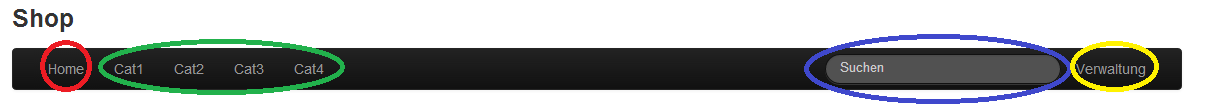
\includegraphics[width=\textwidth]{UserManual/Navi.png}
  \caption{Navigationsleiste}
  \label{fig:Navigationsleiste}
\end{figure}


\section{Produktkatalog}
Zu Beginn des Shopbesuchs oder durch einen Klick auf eine der Schaltflächen Home oder Cat1 bis Cat2 in der Navigationsleiste gelangt man zum Produktkatalog, der alle vorhandenen Produkte darstellt. Ob und auf welche der Schaltflächen geklickt wurde, beeinflusst die Auswahl der angezeigten Produkte. \\
Sollte gerade ein Nutzer angemeldet sein, so werden zusätzlich Empfehlungen prä\-sen\-tiert, die auf seinen gemachten Käufen basieren, sofern vorhanden. Über den Schieberegler darüber kann die Reichweite der Empfehlungen erweitert oder eingeschränkt werden. \\
Durch das Anklicken eines Artikels gelangt man auf dessen Produktbeschreibung (siehe dort).

\begin{figure}[h!]
  \centering
  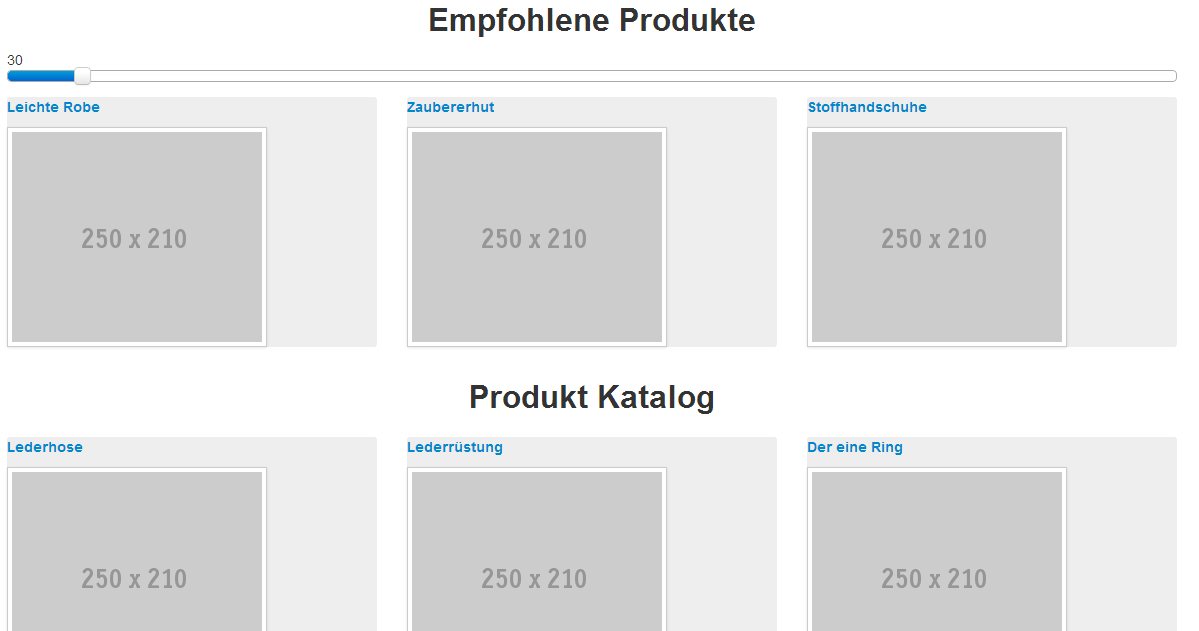
\includegraphics[width=\textwidth]{UserManual/Produktkatalog.png}
  \caption{Produktkatalog}
  \label{fig:Produktkatalog}
\end{figure}


\section{Verwaltung}
Die Administration des Shops kann über das Verwaltungsmenü vorgenommen werden, das über die Navigationsleiste erreichbar ist. Es bietet von oben nach unten die folgenden Funktionen
\begin{itemize}
  \item Produkte verwalten (roter Kreis) \\
        ruft die Produkteverwaltung auf (siehe Abschnitt Produkte)
  \vspace*{-0.5em}
  \item Assoziationen verwalten (grüner Kreis) \\
        ruft die Assoziationsverwaltung auf (siehe Abschnitt Assoziationen)
  \vspace*{-0.5em}
  \item Nutzer verwalten (blauer Kreis) \\
        ruft die Nutzerverwaltung auf (siehe Abschnitt Nutzer)
\end{itemize}

\begin{figure}[h!]
  \centering
  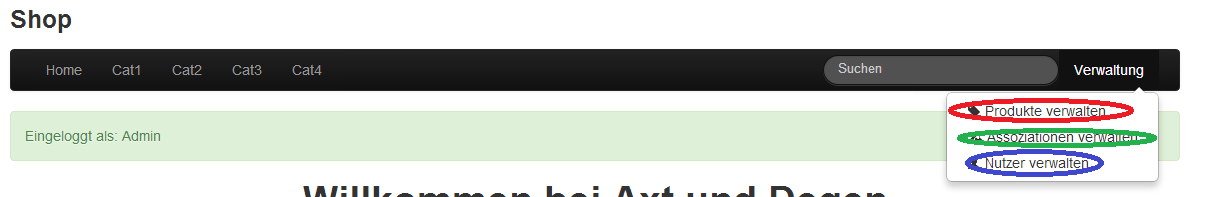
\includegraphics[width=\textwidth]{UserManual/Verwaltung.png}
  \caption{Verwaltung}
  \label{fig:Verwaltung}
\end{figure}


\section{Produkte}
Die Verwaltung der zum Verkauf stehenden Produkte erfolgt über die Produkteverwaltung, die über das Verwaltungsmenü erreichbar ist.  Eine Tabelle listet alle vorhandenen Produkte auf. Die Tabellenzeilen haben von links nach rechts die folgenden Bedeutungen
\begin{itemize}
  \item id \\
        eine eindeutige Identifikationsnummer (generiert nach UUID v4), über die jedes Produkt eindeutig identifiziert werden kann
  \vspace*{-0.5em}
  \item Title \\
        der Name des Produktes
  \vspace*{-0.5em}
  \item Category \\
        die Kategorien des Produktes
  \vspace*{-0.5em}
  \item Sizes \\
        die Größen, in denen das Produkt angeboten wird
  \vspace*{-0.5em}
  \item Colors \\
        die Farben, in denen das Produkt angeboten wird
  \vspace*{-0.5em}
  \item Description \\
        eine Beschreibung des Produktes
\end{itemize}
Jede Tabellenzeile ist anklickbar, um direkt zur entsprechenden Produktbeschreibung (siehe dort) zu gelangen.

\begin{figure}[h!]
  \centering
  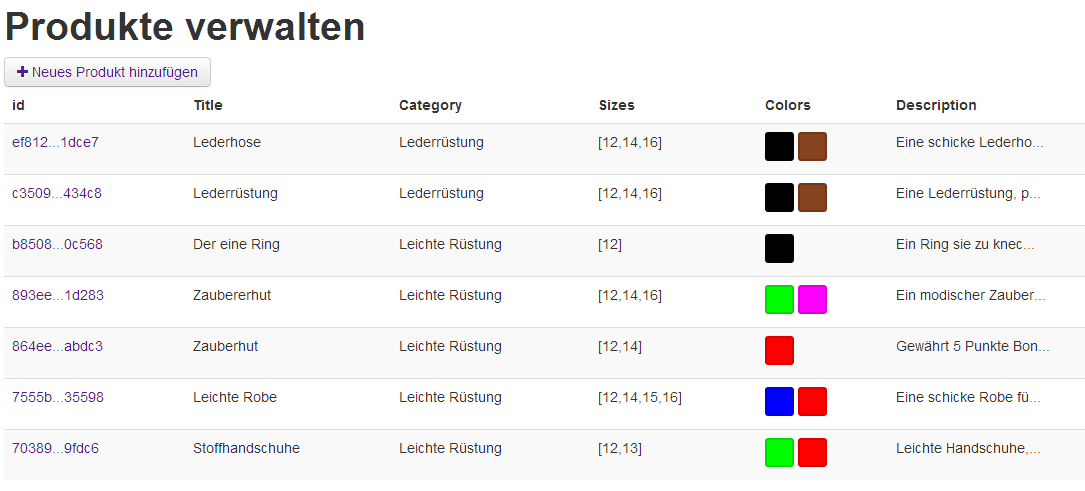
\includegraphics[width=\textwidth]{UserManual/Produkte.png}
  \caption{Produktverwaltung}
  \label{fig:Produktverwaltung}
\end{figure}
\text{}\vspace*{-1em}\\
Über die Schaltfläche Neues Produkt hinzufügen gelangt man zur Produkteeingabemaske, über die neue Produkte in den Shop eingebracht werden können. Dafür müssen alle Felder entsprechend der gewünschten Produktspezifikationen ausgefüllt werden. Von oben nach unten haben sie folgende Bedeutungen
\begin{itemize}
  \item Titel \\
        Name des Produktes
  \vspace*{-0.5em}
  \item Ausrüstungsplatz \\
        Drop-Down-Menü zur Auswahl  des Ausrüstungsplatzes, der von dem Produkt belegt wird
  \vspace*{-0.5em}
  \item Kategorien \\
        kommaseparierte Liste der Kategorien, zu denen das Produkt gehören soll
  \vspace*{-0.5em}
  \item Größen \\
        kommaseparierte Liste der Größen, in denen das Produkt verfügbar sein soll
  \vspace*{-0.5em}
  \item Farben \\
        kommaseparierte Liste der Farben, in denen das Produkt verfügbar sein soll; die Farben müssen in ihren Hexwerten mit führendem ‘\#’ angegeben werden (Bsp: ‘\#ff0000’ für Rot)
  \vspace*{-0.5em}
  \item Beschreibung \\
        eine Beschreibung des Produktes
\end{itemize}
Rechts daneben befinden sich zwei Kästen. Beide beinhalten die vier Attribute Stärke, Intelligenz, Geschicklichkeit und Ausdauer. Die Werte im linken roten Kasten geben die Anforderungen an die Attribute des Nutzers an, um das Produkt verwenden zu können, die Werte im rechten grünen Kasten stellen die Boni auf seine Attribute dar, die der Nutzer durch das Tragen des Produktes erhält.
Mit Betätigen der Schaltfläche Absenden wird das neue Produkt in den Shop übernommen, während ein Klick auf Zurück die Neueingabe abbricht. In beiden Fällen kehrt das Programm auf die Produktverwaltung zurück.


\section{Assoziationen}
Die Kategorien, denen Produkte angehören können, lassen sich mit der Hilfe von Assoziationen koppeln. Dadurch werden Artikel dieser Kategorien als zueinander zu\-ge\-hö\-rig definiert und so in den Produktbeschreibungen (siehe dort) dargestellt. Dies erleichtert es, zusammengehörige Produkte zu erkennen und zu kaufen. Diese Kategorieassoziationen lassen sich in der Assosiationsverwaltung definieren, die über das Verwaltungsmenü erreichbar ist. In dieser werden die vorhandenen Kopplungen in einer Tabelle dargestellt. Durch Klick auf die rote Schaltfläche am Ende einer Tabellenzeile lässt sich die jeweilige Assoziation löschen. \\

\begin{figure}[h!]
  \centering
  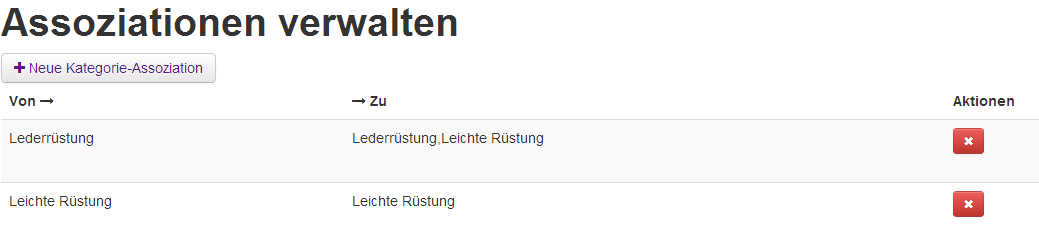
\includegraphics[width=\textwidth]{UserManual/Assoziationen.png}
  \caption{Assoziationen}
  \label{fig:Assoziationen}
\end{figure}
\text{}\vspace*{-1em}\\
Über die Schaltfläche Neue Kategorie-Assoziation gelangt man zur Asso\-zia\-tionen\-ein\-ga\-be\-mas\-ke. Um darüber neue Assoziationen anzulegen, müssen die beiden Felder Von und Zu ausgefüllt werden.  Im ersten Feld wird eine Kategorie eingetragen und im zweiten eine kommaseparierte Liste aus beliebig vielen Kategorien, zu denen eine Kopplung von der Kategorie im ersten Feld aufgebaut werden soll. Kategorien sind nicht automatisch selbstreferenzierend. Soll eine Kategorie sich selbst in einer Assoziation selbst referenzieren, so muss diese ebenfalls im zweiten Feld stehen. Mit Betätigen der Schaltfläche Absenden wird die neu definierte Kopplung übernommen, während ein Klick auf Zurück die Neueingabe abbricht. In beiden Fällen kehrt das Programm auf die Assoziationsverwaltung zurück.


\section{Nutzer}
Die Administration der im Shopsystem registrierten Nutzer erfolgt über die Nutzerverwaltung, die über das Verwaltungsmenü erreichbar ist. Eine Tabelle listet alle im System vorhandenen Nutzer auf. Die Tabellenzeilen haben von links nach rechts die folgenden Bedeutungen
\begin{itemize}
  \item Nutzername \\
        der Name des Nutzers; ist anklickbar, um direkt zu den  Nutzerdetails (siehe unten) zu gelangen
  \vspace*{-0.5em}
  \item Gekaufte Produkte \\
        die Anzahl der von diesem Nutzer gekauften Produkte; ist anklickbar, um direkt zu den Nutzerdetails (siehe unten) zu gelangen
  \vspace*{-0.5em}
  \item Aktionen \\
        drei Schaltflächen, mit denen der Nutzer konfiguriert werden kann (siehe unten)
\end{itemize}
Die drei Schaltflächen haben von links nach rechts die folgenden Funktionen
\begin{itemize}
  \item als entsprechender Nutzer einloggen; ein eventuell bereits eingeloggter anderer Nutzer wird dadurch ausgeloggt (roter Kreis)
  \vspace*{-0.5em}
  \item vollständigen Kauf-Verlauf des Nutzers löschen (grüner Kreis)
  \vspace*{-0.5em}
  \item Nutzer löschen (blauer Kreis)
\end{itemize}

\begin{figure}[h!]
  \centering
  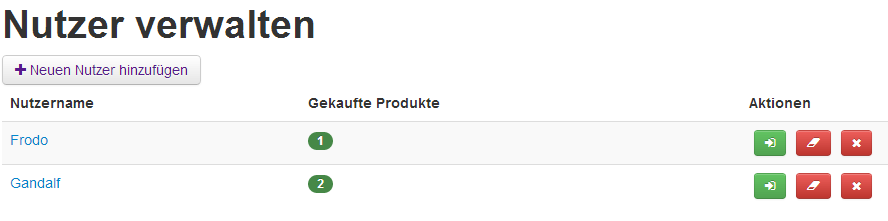
\includegraphics[width=\textwidth]{UserManual/Nutzer.png}
  \caption{Nutzer}
  \label{fig:Nutzer}
\end{figure}
\text{}\vspace*{-1em}\\
Die Nutzerdetails zeigen die Attribute des Nutzers und Kaufhistorie an. Über die Schaltfläche oberhalb der Attributwerte können diese geändert werden. Die Bedeutungen der Spalten der Tabelle der gekauften Produkte entsprechen den gleichnamigen Spalten der Tabelle aus der Produkteverwaltung (siehe Abschnitt Produkte). Durch einen Klick auf die Löschen-Schaltfläche in der Spalte Actions wird das dazugehörige Produkt gelöscht.  Die Produkttitel sind anklickbar und führen direkt zur dazugehörigen Produktbeschreibung (siehe dort).

\begin{figure}[h!]
  \centering
  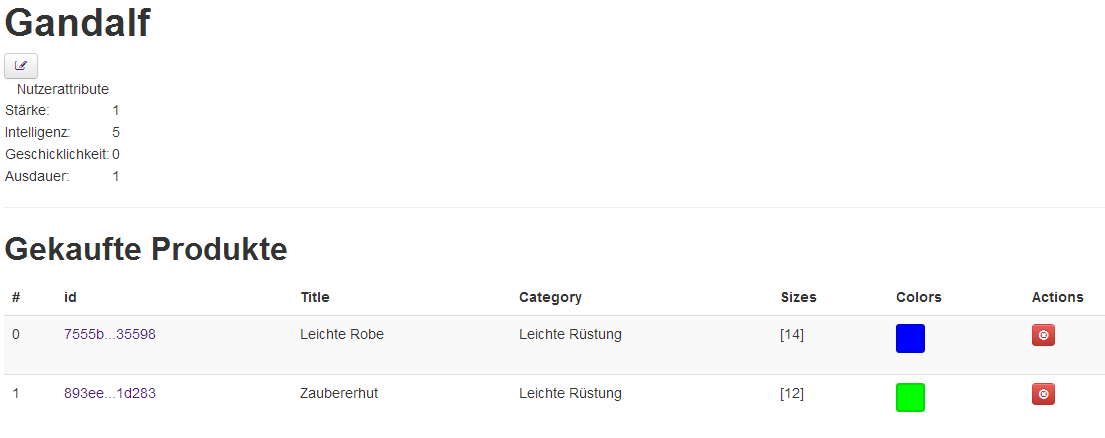
\includegraphics[width=\textwidth]{UserManual/Nutzerdetails.png}
  \caption{Nutzerdetails}
  \label{fig:Nutzerdetails}
\end{figure}
\text{}\vspace*{-1em}\\
Über die Schaltfläche Neuen Nutzer hinzufügen gelangt man zur Nutzereingabemaske, über die neue Nutzer im System registriert werden können. Dafür müssen alle Felder ausgefüllt werden. Sie haben folgende Bedeutungen
\begin{itemize}
  \item Name \\
        Name des Nutzers
  \vspace*{-0.5em}
  \item Stärke, Intelligenz, Geschicklichkeit, Ausdauer \\
        die Höhe des jeweiligen Attributwertes des Nutzers
\end{itemize}
Mit Betätigen der Schaltfläche Absenden wird der neue Nutzer in das System übernommen, während ein Klick auf Zurück die Neueingabe abbricht. In beiden Fällen kehrt das Programm auf die Nutzerverwaltung zurück.


\section{Produktbeschreibungen}
Jedes Produkt besitzt eine eigene Seite, durch die es präsentiert wird. Außerdem kann es über diese gekauft werden. Jede Produktbeschreibung besteht aus den folgenden Bestandteilen
\begin{itemize}
  \item Titel (roter Kreis)
  \vspace*{-0.5em}
  \item Bild des Produktes (gelber Kreis)
  \vspace*{-0.5em}
  \item Beschreibung des Produktes (schwarzer Kreis)
  \vspace*{-0.5em}
  \item durch das Tragen des Produktes gewährte Attributsboni  (grüner Kreis)
  \vspace*{-0.5em}
  \item Ausrüstungsplatz, an dem das Produkt getragen wird (hellblauer Kreis)
  \vspace*{-0.5em}
  \item Attributswerte, die ein Nutzer besitzen muss, um das Produkt tragen zu können (lila Kreis)
  \vspace*{-0.5em}
  \item Drop-Down-Menü, um die gewünschte Größe auszuwählen (brauner Kreis)
  \vspace*{-0.5em}
  \item Radioboxen, um die gewünschte Farbe auszuwählen (rosa Kreis)
  \vspace*{-0.5em}
  \item Schaltfläche zum Kaufen des Produktes (grauer Kreis)
  \vspace*{-0.5em}
  \item mit dem aktuellen Produkt in Verbindung stehende andere Artikel (dunkelblauer Kreis)
\end{itemize}
Um ein Produkt zu erwerben, müssen erst Größe und Farbe ausgewählt werden, bevor die Kaufen-Schaltfläche bestätigt wird. Ansonsten erscheint eine Fehlermeldung. Durch Klicken auf die zugehörigen Produkte wird zu deren jeweiliger Produktbeschreibung gewechselt.

\begin{figure}[h!]
  \centering
  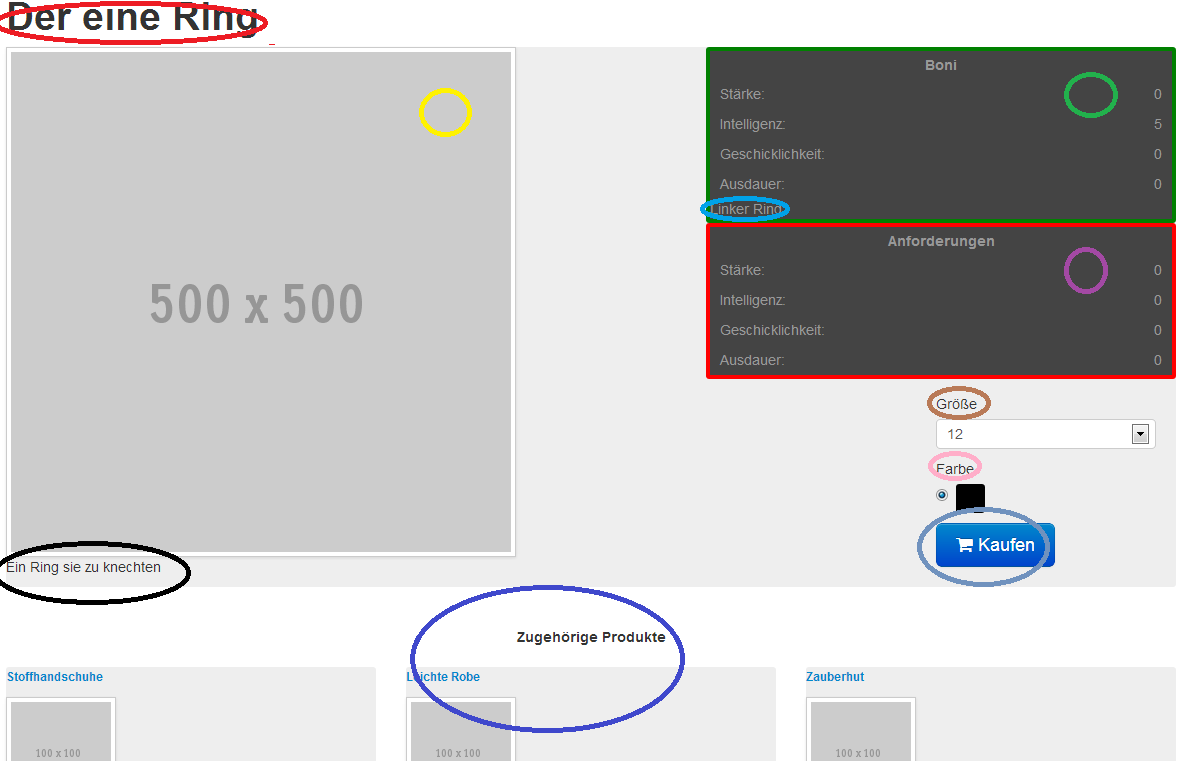
\includegraphics[width=\textwidth]{UserManual/Produktbeschreibung.png}
  \caption{Produktbeschreibung}
  \label{fig:Produktbeschreibung}
\end{figure}


\section{StateManager}
Zusammen mit der Shopsoftware wird das Programm StateMananger ausgeliefert. Mit seiner Hilfe können die Produkte und Assoziationen in der Shopdatenbank auch bei nicht laufendem Server betrachtet werden. Außerdem können diese im \textsf{JSON}-Format exportiert oder importiert werden. Dies erlaubt eine einfache Übertragung des Shops auf neue Systeme. Die exportierten Dateien finden sich im Ordner sample im \textsf{ecom}-Verzeichnis. \\
Der StateManager lässt sich über die Kommandozeile aus dem ecom-Verzeichnis heraus bedienen. Der Befehl \textsf{runhaskell -isrc tools/StateManger.hs --help} liefert weitere Informationen zu seiner Benutzung. 